\documentclass[a4paper,12pt]{article}

\usepackage[danish]{babel}
\usepackage[utf8]{inputenc}
\usepackage[pdftex]{graphicx}
\usepackage{subfigure}
\usepackage{usecases}
\usepackage{setspace}
\onehalfspacing
\usepackage{upquote}
\usepackage{color}
\definecolor{listinggray}{gray}{0.9}
\usepackage{listings}
\lstset{
	language=,
	literate=
		{æ}{{\ae}}1
		{ø}{{\o}}1
		{å}{{\aa}}1
		{Æ}{{\AE}}1
		{Ø}{{\O}}1
		{Å}{{\AA}}1,
	backgroundcolor=\color{listinggray},
	tabsize=3,
	rulecolor=,
	basicstyle=\scriptsize,
	aboveskip={1.5\baselineskip},
	columns=fixed,
	showstringspaces=false,
	extendedchars=true,
	breaklines=true,
	prebreak =\raisebox{0ex}[0ex][0ex]{\ensuremath{\hookleftarrow}},
	frame=single,
	showtabs=false,
	showspaces=false,
	showstringspaces=false,
	identifierstyle=\ttfamily,
	keywordstyle=\color[rgb]{0,0,1},
	commentstyle=\color[rgb]{0.133,0.545,0.133},
	stringstyle=\color[rgb]{0.627,0.126,0.941},
}
\usepackage[center,font=small,labelfont=bf,textfont=it]{caption}
\usepackage{enumerate}
\usepackage[numbers]{natbib}
\usepackage{hyperref}
\hypersetup{
	pdfborder = {0 0 0},
    colorlinks,
    citecolor=blue,
    filecolor=blue,
    linkcolor=blue,
    urlcolor=blue
}
\usepackage{parskip}
\setlength{\parindent}{15pt}

\begin{document}

\begin{titlepage}


\newcommand{\HRule}{\rule{\linewidth}{0.5mm}} % Defines a new command for the horizontal lines, change thickness here

\center % Center everything on the page

\textsc{\LARGE Københavns Universitet}\\[1.5cm] % Name of your university/college
\textsc{\Large Projektkursus Systemudvikling 2014}\\[0.5cm] % Major heading such as course name

\HRule \\[0.4cm]
{  \bfseries \large Open Source Bannerreklamesystem \\ \huge EasyAd}\\[0.4cm] % Title of your document
\HRule \\[1.5cm]

\begin{minipage}[t]{0.4\textwidth}
\begin{flushleft} \large
\emph{Projektgruppe:}


Signar Nielsen % Your name
\\
060585
\newline
\\
Aslak Niclasen
\\
060693
\newline
\\
Amanda Bergqvist
\\
171090
\end{flushleft}
\end{minipage}
~
\begin{minipage}[t]{0.4\textwidth}
\begin{flushright} \large
\emph{Instruktor:} \\
Aske Mottelson Clausen % Supervisor's Name
\end{flushright}
\end{minipage}\\[4cm]

{\large 24. april 2014}\\[3cm] % Date, change the \today to a set date if you want to be precise

\end{titlepage}

\tableofcontents %generate table of content


\clearpage %clears float-buffer - inserting those missing - and starts new page

\section{Indledning}
Ifølge en rapport fra Danske Medier Research\footnote{\url{ http://www.fdim.dk/sites/default/files/mediearkiv/rapporter/danskernes\_brug\_af\_internettet\_2012\_rapport.pdf}} om danskernes internetforbrug er adgang til internettet fra hjemmet steget fra 83\% til 92\% på blot 4 år - fra 2007 til 2011. I takt med den stigende grad af internetforbrug anvender annoncører de digitale medier til at ramme deres målgruppe.

Flere og flere virksomheder, interesseorganisationer og foreninger bliver derfor synlige på internettet med en hjemmeside eller profil på de sociale medier. De står alle overfor samme udfordring, nemlig hvordan man tjener penge på nettet. Den mest udbredte forretningsmodel er salg af annoncer på nettet. Der er to udfordringer ved at annoncere på nettet; den ene er den tekniske udfordring ved at selv skulle vedligeholde et bannersystem, og den anden er den økonomiske udfordring ved at skulle købe sig adgang til et bannersystem eller den nødvendige tekniske viden. Vores system er et forsøg på at løse disse to problemer.

\section{Abstract}

Projektet Easy Ad er et open source bannerreklamesystem. Formålet med Easy Ad er at udvikle et systemet der er nemt og gratis at bruge. Systemet skal kunne downloades af mindre ikke-kommercielle foreninger og interesseorganisationer, der hverken har de fornødne midler til at købe dyre systemer eller den tekniske viden til at vedligeholde et sådan system.

Easy Ad skal udvikles til et firma ved navn Treu Media. Treu Media er specialiceret indenfor annoncesalg og en lang række andre medieudgivelser. Easy Ad skal gøre det nemt for Treu Media at administrere annoncer til deres mange kunder. Systemet skal derudover løse en lang række tekniske udfordringer, som f.eks. hvordan man sikrer med hvilken vægtning et banner bliver vist. Eller hvordan man undgår at samme banner bliver vist flere gang på samme hjemmeside.

Simon Shine er den tekniske kontaktperson og det er ham der sætter de tekniske krav til systemet. Jan Treu-Nielsen, Treu Media's ejer, vil være kontaktperson ved aftesting og opsætning af systemet. Projektet vil løbe fra marts og indtil ultimo juni. Systemet er en prototype og vil muligvis ikke være færdig udviklet ved projektets udgang. 

\section{IT-projektets formål og rammer}

Projektet har til formål at udvikle et open source bannerreklamesystem. Nedenfor ses projektets overordnede rammer og formål beskrevet i faktor-kriteriet. 

\subsection{FACTOR-kriteriet}

\large{\bf{F}}\normalsize{unctionality
\\
- Visning af bannere med forskellig vægtning
\newline
- Tidsbestemt/antalsbestemt bannervisning 
\newline
- Oprettelse af kunder 
\newline
- Oprettelse af grupper
\newline
- Oprettelse af bannere}
\newline
\newline
\large{\bf{A}}\normalsize{pplication domain
\\
- Medarbejdere tilknyttet Treu media}
\newline
\newline
\large{\bf{C}}\normalsize{onditions\\
- Skal kunne bruges på tværs af browsere\\
- Skjult for brugere af hjemmesider\\
- Open source}
\newline
\newline
\large{\bf{T}}\normalsize{echnology\\
- Web-teknologi: html, css, php, javascript.\\
- Databaser: MySQL\\
- Webserver: Apache}
\newline
\newline
\large{\bf{O}}\normalsize{bjects\\
- Bannere/Reklamer
\newline
- Administratorer
\newline
- Kunder
\newline
- Grupper}
\newline
\newline
\large{\bf{R}}\normalsize{esponsibility\\
- Holder styr på banner visning}

\section{Kravspecifikation for IT-løsningen}
\subsection{Funktionelle og ikke-funktionelle krav}
\textbf{Funktionelle krav}
\\
Funktionelle krav beskriver interaktionen mellem brugeren og systemet - uden at systemet fysisk, eller i praksis, er implementeret. Funktionelle krav siger noget om, hvordan systemet skal fungere, forventet input til systemet og forventet output fra systemet. De praktiske, eller fysiske, krav til systemet er beskrevet i ikke-funktionelle krav nedenunder.

EasyAd er et system, som gør det muligt at vedligeholde reklamer på en hjemmeside. Systemet er opbygget sådan, at det kan være ejeren der administrerer systemet, eller det er en tredje part, der administrerer systemet. Dette gør, at man altid skal kunne logge på for at få adgang til systemet og for at kunne administrere reklamerne. Når man er logget på systemet, skal man oprette en hjemmeside (eller en kunde), hvor reklamen skal vises, og derefter skal man oprette en gruppe (eller en zone), som reklamen hører til. Til sidst skal man oprette selve reklamen og tilføje den til en gruppe.

Hjemmesiden (eller kunden), der oprettes kan være ens egen hjemmeside, eller det kan være kundens hjemmeside. I begge tilfælde skal hjemmesiden have adgang til systemet via en API, for at få vist en hjemmeside.

Grupperne bestemmer, hvor på siden, reklamen skal vises. Hvis man f.eks. kun ønsker at få en reklame vist på en underside, kan man lave en gruppe til undersiderne, mens man har en anden gruppe til forsiden.
\\
\\
\textbf{Ikke-funktionelle krav}
\\
Ikke-funktionelle krav er direkte krav til systemet, hvor og hvordan det skal fungere. Ikke-funktionelle krav bliver også kaldt kvalitets krav, det vil sige krav til kvaliteten af det system, eller program, man udvikler. Man kan f.eks. stille krav til performance, pris, sikkerhed og mange andre ting. 

Da ikke-funktionelle krav er et vidt begreb, har vi valgt at bruge FURPS+ modellen, som bogen også bruger. FURPS står for Functionality, Usability, Reliability, Performance and Supportability. Plusset står for under-kategorier, som også bliver kaldt constraints.

Her er de ikke-funktionelle krav:
\begin{itemize}
	\item \textbf{Functionality:} Systemet skal kunne håndtere (oprette, ændre og vise) reklamer på en hjemmeside. Dette kræver selvfølgelig, at alle involverede parter har adgang til internettet. Det vil sige, systemet, hjemmesiden og brugeren af hjemmesiden.
	\item \textbf{Usability:} Formålet med systemet er, at det skal være nemt at bruge for alle involverede parter. Både administratorer, hjemmesider og brugere. Da det er meget svært at definere, hvad er "nemt" at bruge, laver vi nogle user-tests, for at sikre os, at det faktisk er nemt at bruge. Da tiden og resourcerne er begrænsede, vil vi ikke teste, om systemet er nemt at sætte op. Vi er nødt til at prioritere, og derfor vil vi i stedet teste, om systemet er nemt at bruge, efter det er blevet sat op. Dette vil vi teste sammen med Treu Media, hvor vi vil lave et tænk-højt eksperiment. Det er også vigtigt, at systemetet fungerer på alle moderne browsere (IE8+, Safari, Chrome og Firefox). Dette kan nemt testes i f.eks. browserstack.com - hvis der er tid til det, vil vi udføre sådan en test.
	\item \textbf{Reliability:} Denne del er lidt udenfor vores kontrol, da vi ikke kan styre, hvor og i hvilket miljø systemet vil blive sat op. Der skal ikke være nogen software-forhindring for, at systemet skal kunne være tilgængeligt 24 timer i døgnet 365 dage om året. Hvis vi antager, at serveren altid har forbindelse til internettet, så sætter dette først og fremmest krav til serveren, både hardware og software. Serveren skal være dimensioneret til at kunne håndtere trafikken og softwaren skal være designet på en hensigtsmæssig måde, så den ikke bruger unødvendige resourcer.
	\item \textbf{Performance:} Det er et krav til systemet, at svartiden er så lav som overhoved muligt. Der er flere faktorer, der spiller ind, men først og fremmest er det internetforbindelsen, serveren og selve softwaren. Brugen skal ikke bemærke, at han venter på, at reklamerne loader. Dette kan gøres på forskellige måder, f.eks. ved at loade reklamerne asynkront ved hjælp af XHR-objektet i JavaScript, så siden bliver mere brugervenlig.
	\item \textbf{Supportability:} Systemet kan understøttes af enhver, da det er open-source. Systemet bliver udviklet i PHP, hvilket også er et open-source sprog.
\end{itemize}

\textbf{Constraints:} Systemet er webbaseret og vil blive udviklet i PHP. Derudover benytter vi andre webteknologier, som f.eks. HTML, CSS, JavaScript (jQuery). Projektet er open-source, men hvis man vil udvikle, eller udvide, systemet, kan man gøre det i PHP. Vi har valgt at benytte en MySQL-database. I forhold til reklamerne skal man kunne uploade almindelige billeder, videosekvenser og flash-filer. Vi har ikke taget en endelig stilling til, hvilke filtyper man skal have lov til at uploade.

\subsection{Højniveau use case model}
Vi har lavet et højniveau use case diagram, som viser aktørerne og systemets funktionalitet. Treu Media har mulighed for at administrere kunder, grupper og reklamer, mens kunden (som også kan være en besøgende på en hjemmeside), får vist en reklame.

\begin{figure}[h!]
  \centering
    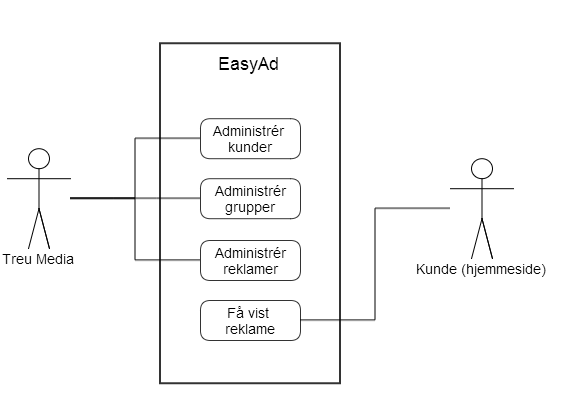
\includegraphics[scale=0.5]{use_case.png}
  \caption{Højniveau use case model}
\end{figure}

\subsection{Tre use case modeller}
Vi har en interessent, som er Treu Media, som har fået en ny kunde og har solgt et banner til kunden. Nu skal Treu Media oprette kunden i systemet, oprette en gruppe og oprette en reklame.

\begin{figure}[h!]
  \centering
    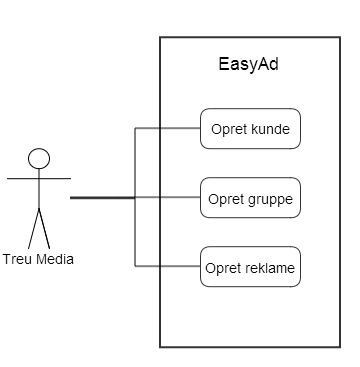
\includegraphics[scale=0.5]{three_use_cases.png}
  \caption{Administrator skal oprette en reklame}
\end{figure}

Vi starter med den første use case, hvor administrator skal oprette en kunde:
\begin{usecase}
\addtitle{Use case navn:}{Opret kunde}
\addfield{Aktør:}{Treu Media}
\addscenario{Flow:} {
	\item Tryk på "Customers"
	\item Tryk på "Add customer"
	\item Udfyld felterne "Name" og "Url". Begge felter skal udfyldes
	\item Tryk på "Submit"
}
\addfield{Startbetingelser:}{Treu Media skal være logget på systemet}
\addfield{Slutresultat:}{En kunde er oprettet i systemet}
\end{usecase}

Derefter tager vi en use case, hvor administrator skal oprette en gruppe, som tilhører en kunde:
\begin{usecase}
\addtitle{Use case navn:}{Opret gruppe}
\addfield{Aktør:}{Treu Media}
\addscenario{Flow:} {
	\item Opret en kunde. Se tidligere use case
	\item Tryk på "Groups"
	\item Tryk på "Add group"
	\item Udfyld feltet "Group name" og vælg en kunde fra select-boksen
	\item Tryk på "Create"
}
\addfield{Startbetingelser:}{Treu Media skal være logget på systemet. Der skal være oprettet en kunde}
\addfield{Slutresultat:}{En gruppe er oprettet i systemet}
\end{usecase}

Til sidst tager vi en use case, hvor administrator skal oprette en reklame, der tilhører en gruppe.
\begin{usecase}
\addtitle{Use case navn:}{Opret reklame}
\addfield{Aktør:}{Treu Media}
\addscenario{Flow:} {
	\item Opret en kunde. Se tidligere use case
	\item Opret en gruppe. Se tidligere use case
	\item Tryk på "Ads"
	\item Tryk på "Add ad"
	\item Udfyld feltet "Ad name" og vælg en kunde fra select-boksen og vælg siden, hvilken gruppe reklamen skal høre til fra select-boksen
	\item Vælg reklamen fra din computer ved at trykke på "Vælg fil"
	\item Tryk på "Submit"
}
\addfield{Startbetingelser:}{Treu Media skal være logget på systemet. Der skal være oprettet en kunde og en tilhørende gruppe.}
\addfield{Slutresultat:}{En reklame er oprettet i systemet}
\end{usecase}

\subsection{Klassediagram}
Vores klasser er følgende: administrator, kunde, gruppe og reklame. Forholdet mellem klasserne er, at flere grupper kan tilhøre én kunde og flere reklamer kan tilhøre én gruppe. Derved kan flere reklamer også tilhøre én kunde.

\begin{figure}[h!]
  \centering
    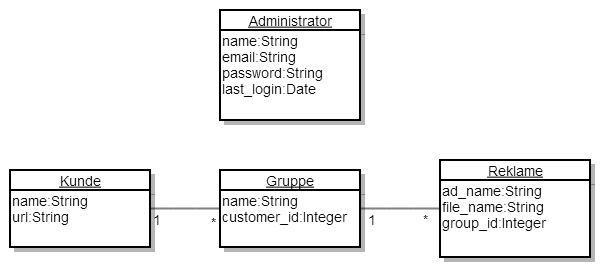
\includegraphics[scale=0.5]{klasse_diagram.png}
  \caption{Klassediagram}
\end{figure}

\section{Systemdesign sammenfatning}
Vi er nået dertil, at Treu Media kan oprette kunder, grupper og reklamer. Vi har lavet en grov skitse af systemet, men mangler at implementere nogle funktioner, som f.eks. at give Treu Media mulighed for at ændre en kunde, gruppe og reklame. Vi skal også sørge for at beskytte imod SQL-injections og sikre os, at de krævede felter faktisk bliver udfyldt, når Treu Media f.eks. opretter en reklame. Den vigtigste funktion vi mangler, er at vise en reklame på en hjemmeside. Der findes flere muligheder for, hvordan vi kan lave denne del af systemet. Vi har diskuteret fordele og ulemper ved de forskellige muligheder, og har ikke truffet en endelig beslutning. Højst sandsynligt vælger vi en løsning, hvor kunden skal tilføje en javascript-fil til hjemmesiden, som henter og placerer reklamerne på hjemmesiden.

\section{Program- og systemtesting}

Projektgruppen ønsker at teste systemet i flere omfang. Disse omhandler både interne og eksterne kravspecifikationer.

\subsection{Interne test}
Ved de interne test skal vi benytte os af unit testing. Denne testing skal finde sit ståsted i matematikken, og vil omhandle en form for tællemekanisme. Gruppen ønsker længere fremme i projektet at teste antallet af visninger af bannere på hjemmesider. Vi skal altså forsøge at skabe en bannervisning internt i programmet et kendt antal gange. Vores tællemekanisme skal således beregne et resultat udfra vores banneres visning. Dette resultat skal herefter sammenlignes med det forventede antal visninger fra start.

En konkret måde at løse gruppens problem her, kunne være på følgende måde: uploade et banner, sende fiktive requests til en hjemmeside med dette banner. Herved kunne gruppens tællemekanisme aflæse om requesten bliver behandlet korrekt og dermed registrere en visning. Dette ville resultere i at man kan tælle antallet af requests som der er blevet behandlet i processen og gruppen ville hurtigt kunne se om det forventede resultat stemte overens med det relle resultat fra vores tællemekanisme.

\subsection{Eksterne test}
Projektgruppen regner desuden med testing af systemets nuværende GUI. Gruppen forsøger at skabe et "tænke højt forsøg" som indebærer at interessenten benytter sig af systemet. Vi vil på forhånd give interessenten systemet i hænderne, og guide denne i en retning med henblik på testing af brugervenligheden og korrekthed af vores GUI. Der vil på forhånd være stillet en række opgaver, som i projektgruppens øjne er set som de væsentligste faktorer for systemets kunnen (use cases). Disse små opgaver skal interessenten dernæst udføre, eller prøve at udføre på egen hånd. En form for dokumentering behøves. 

Da projektgruppen ikke burde være til stede under testingen af programmet, ville man benytte sig af f.eks. videooptagelse så interessenten kunne afprøve systemet uden vores indflydelse eller kommentarer om systemet. Herved ville vi få et bedre overblik og en viden om hvordan mennesker håndterer systemets kunnen.
Under dette forsøg ville de eksterne kravspecifikationer uden tvivl komme i spil. F.eks. brugervenlighed ift. overblik fra
interessentens side.

\section{Brugergrænseflade og interaktionsdesign}
\subsection*{Skærmbilleder}
\textbf{Oversigt og oprettelse af kunde}
\begin{figure}[h!]
  \centering
    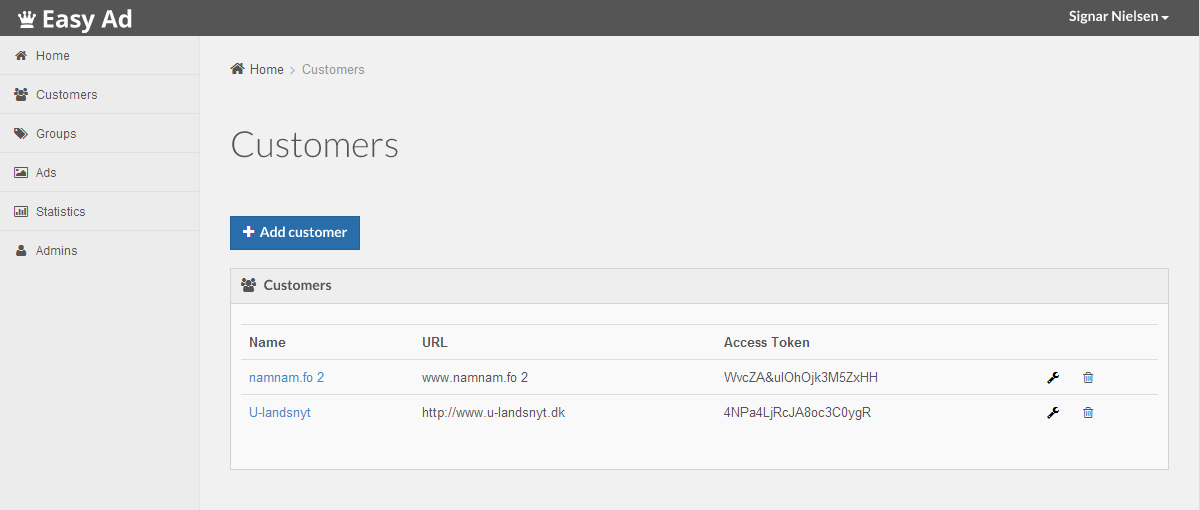
\includegraphics[width=\textwidth]{customers.png}
  \caption{Oversigt over kunder}
\end{figure}

\begin{figure}[h!]
  \centering
    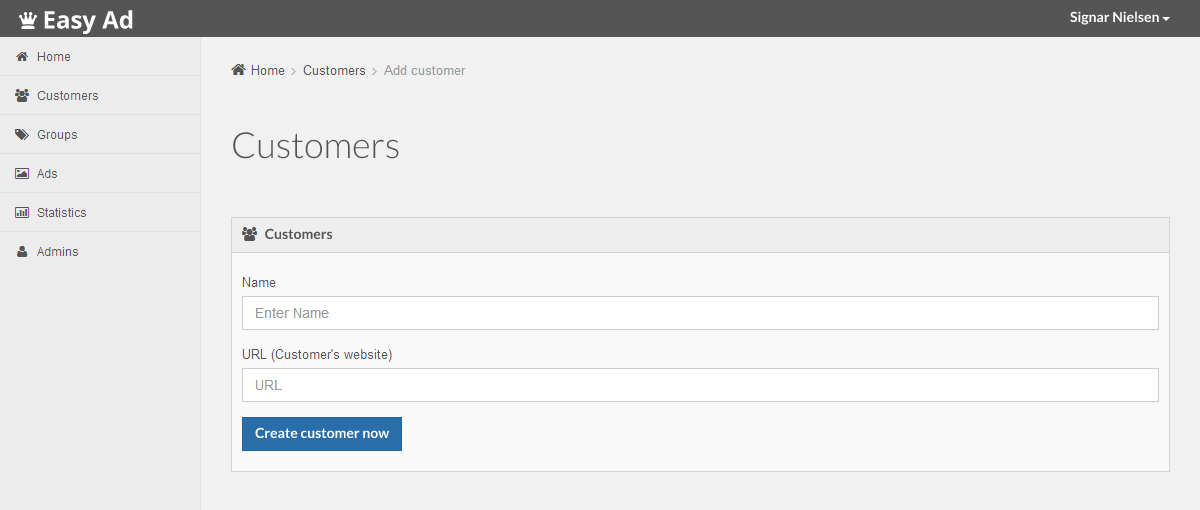
\includegraphics[width=\textwidth]{customer_add.png}
  \caption{Oprettelse af kunde}
\end{figure}

\textbf{Oversigt og oprettelse af reklamer}
\begin{figure}[h!]
  \centering
    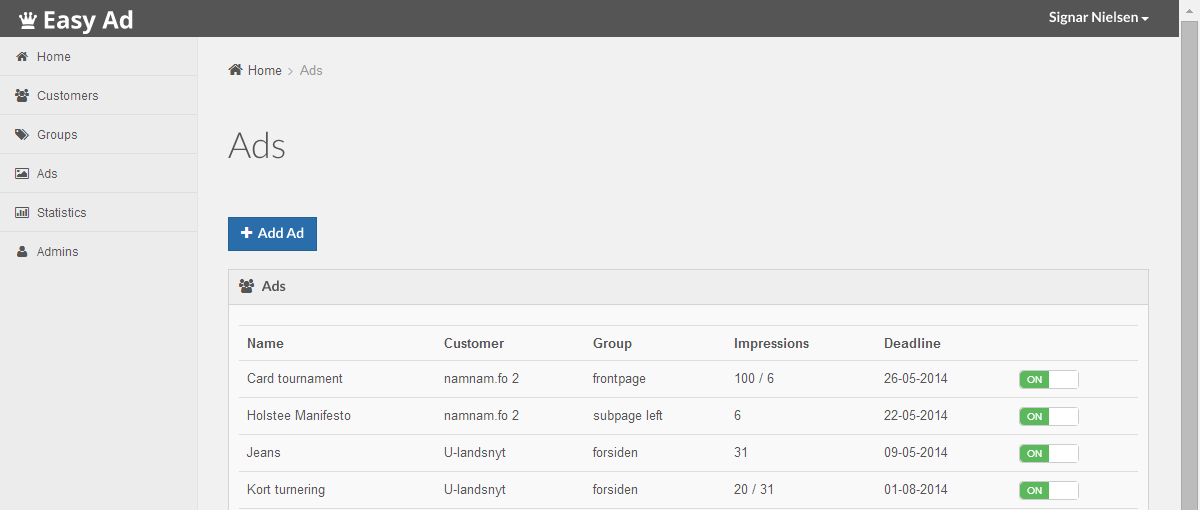
\includegraphics[width=\textwidth]{ads.png}
  \caption{Oversigt over reklamer}
\end{figure}

\begin{figure}[h!]
  \centering
    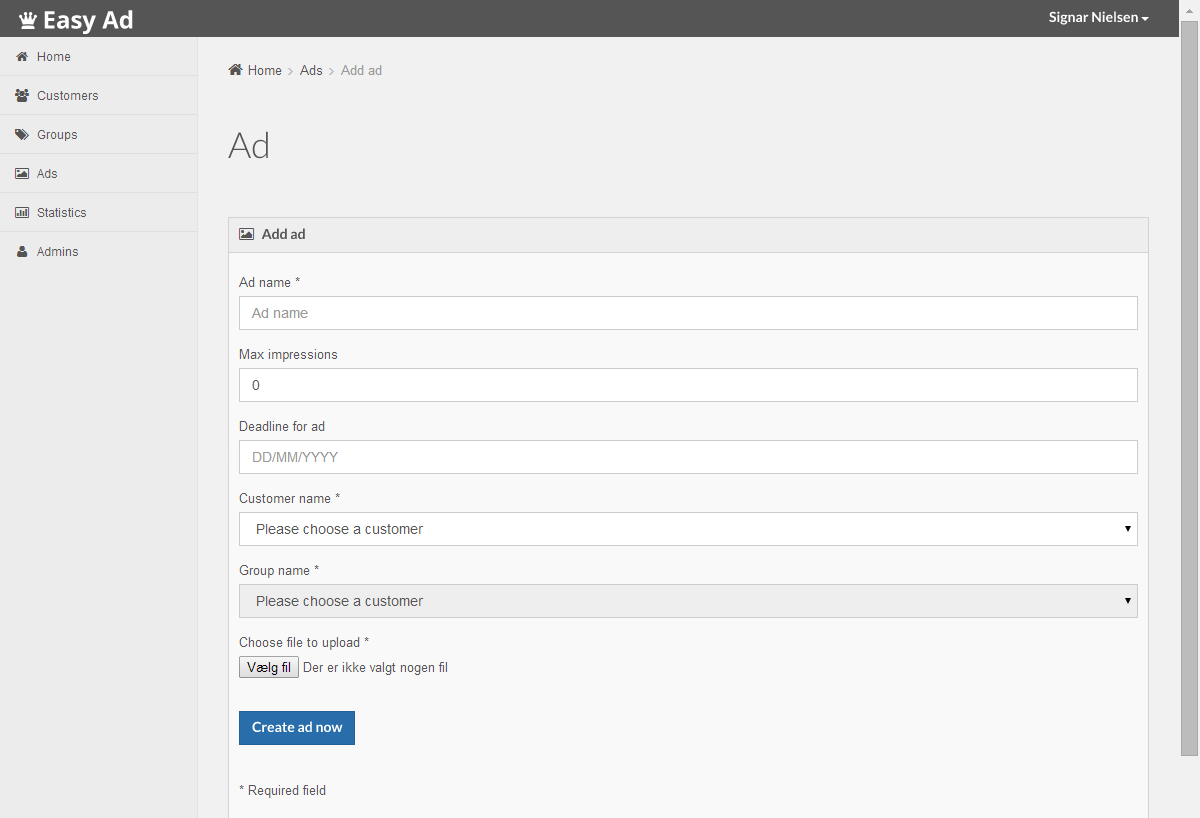
\includegraphics[width=\textwidth]{ad_add.png}
  \caption{Oprettelse af reklame}
\end{figure}

\textbf{Statistik for reklamer}
\begin{figure}[h!]
  \centering
    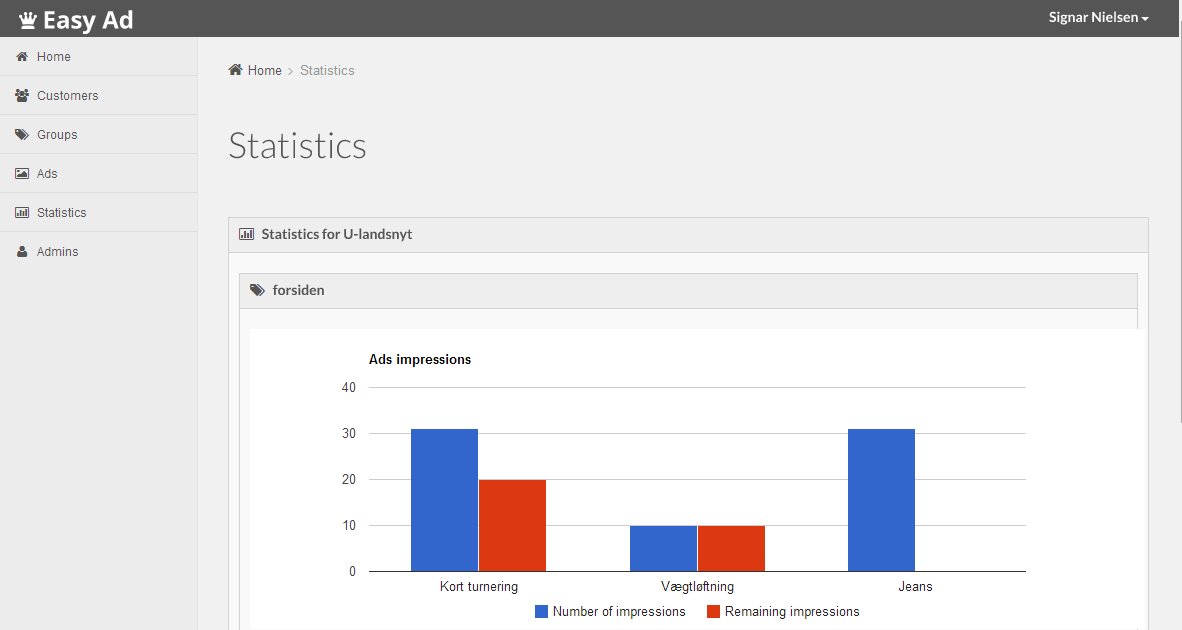
\includegraphics[width=\textwidth]{statistics.png}
  \caption{Statistik for reklamer}
\end{figure}

\newpage
\subsection*{Audio visuel præsentation}
Vi har lavet en demonstration af vores brugergrænseflade, som vi har uploaded til youtube:
\newline
\url{www.youtube.com/watch?v=RXtx08uCdH4&feature=youtu.be&hd=1}

\subsection*{Tænke-højt forsøg}
Vi har ikke udført et tænke-højt forsøg endnu, men det har vi planer om at nå til næste rapport.

\section{Versionstyring}
Vi benytter GitHub til versionstyring. Vores projekt ligger på
\newline
\url{http://github.com/AslakNiclasen/ProjektOpgave}.
\newline
\\
Da vi commiter flere gange i løbet af en programmerings-session, giver det ikke rigtig nogen mening at vedhæfte vores commit-log fordi den er så lang. Den er også offentlig, så alle kan gå ind og se den. Vi har hellere ikke valgt at vedhæfte vores kode, da den også er offentlig.
\newline
\\
Vi har valgt at commite tit, så vi undgår risikoen ved at den stor del af arbejdet går tabt, hvis uheldet er ude. Grunden til, at Aslak ikke har commited lige så ofte, som de andre er fordi, at han har problemer med Git på sin computer.


\section{Projektsamarbejdet}
\subsection{Hvad går godt?}

\textbf{Internt}
\newline
Projektgruppen har i løbet af påsken mødtes en gang om ugen, og disse har været meget produktive. Til disse møder har vi haft en dagsorden, vi har planlagt små arbejdsopgaver frem til næste mødes dagsorden og vi har planlagt opgaveskrivning individuelt. Arbejdet mellem gruppen internt, fungerer meget gnidningsfrit og alle opfylder hindandens krav, og de krav der stilles til opgaven. Alle møder velforberedte og friske, således at dagen hvor vi alle har mulighed for at mødes bliver så konstruktiv som overhoved muligt.

Det var en smule kompliceret at finde en god mødefordeling i påskeferien, da alle 3 medlemmer havde personlige ærinder der skulle imødekommes. Det har gjort at vi til dels har været tvunget til at skrive anden delrapport i punkter individuelt hver for sig. Vi mødes af den grund mandagen inden aflevering til korrektur læsning, og forståelses/formidlingsmæssige usikkerheder. Alle i gruppen er blevet tildelt ca. lige meget rapportskrivning, så ingen i gruppen føler sig overbebyrdet, eller omvendt, overset. 
\\
\\
\textbf{Med interessent}
\\
Vi har ikke haft et møde med vores interessent til dags dato, men vi har haft 2 møder og mailkorrespondance til vores mellemled mellem os og interessenten. Interessenten giver klart udtryk for et frugtbart samarbejde, med mulighed for fremtidige møder efter vores ønske - det kommer vi selvfølgelig til at benytte os 
af.

Vi har på nuværende tidspunkt en GUI som fungerer efter hensigten, og dette er også grunden til at vi ikke ville mødes med interessenten inden. Projektgruppen ønskede at have noget brugbart rent fysisk at vise frem, således at interessenten ville have nemmere ved at sætte sig ind i projektets omfang, og herunder forstå projektet. Dvs. at vi til dette møde kunne fremsætte klare retningslinier med det fokus at interessenten ville kunne udføre et "tænke højt forsøg" (testing af GUI) og hermed danne sig et billede af systemet. Vi ville af dette opnå stor viden, da vi med en kontrolleret testing af vores system kan fusionere tekniske aspekter med menneskelige input.

Med denne viden kunne vi vidreudvikle vores system, således at der måske sættes fokus på brugervenlighed, eller andet. Det er op til os og interessenten i sammarbejde.
\\
\\
\subsection{Hvad går mindre godt?}

\textbf{Internt}
\\
Som benævnt i punktet ovenover, ville det være mere hensigtsmæssigt at mødes flere gange i påsken. Men det har desværre ikke været muligt. Vi synes dog at vi har fået det optimale ud af vores sammarbejde.
Et medlem i gruppen havde store problemer med github, eftersom hans system er Mac OS X. Det gjorde at han måtte ty til andre løsningsmidler og gruppen har således ikke mistet nogle former for data. Men man blev derfor tvunget til at sende stoffet til de andre medlemmer i gruppen således at de kunne overføre data til github som planlagt. Derfor ses det også i "contributions" fra denne person. Heldigvis burde problemet være løst med en virtuel maskine som benytter Windows på personens Mac OS X i stedet for.
\\
\\
\textbf{Med interessent}
\\
I og med at gruppen ikke har haft møde med interessenten, er det svært at foretage en vurdering af dette punkt. Vi synes dog i og med at interessenten viser meget interesse og er nem at få kontakt til telefonisk, at vi ikke har nogen problematik her. 
\\
\\
\subsection{Hvilke optimeringer i forhold til projektarbejdet kan vi foretage?}

\textbf{Internt}
\\
Vi vil holde lidt flere møder fremover, alt efter behov. Gruppen arbejder velfungerende i det mønster som den har sat sig i pt. Så planlægningen og strukturen af arbjedet forbliver uændret indtil videre.
\\ 
\\
\\
\textbf{Med interessent}
\\
Gruppen begynder planlægning fremover telefonisk med interessenten, og så vil der fra møde til møde indgå klare dagsordner hvis projektet skal fungere optimalt når gruppen skal diskutere emner mere dybdegående med denne.  

\newpage
\pagenumbering{gobble}
\section{Bilag 1 - Review: A rational design process}
Artiklen beskriver den rationelle design process og hvorledes denne er uopnåelig. Dette skyldes i høj grad uvished og menneskelige fejl, men problemet opstår også ved komplexiteten af store programmer. Denne komplexitet gør det svært at overskue processen og alle dens detaljer, hvilket fører til menneskelige fejl. Man kan løse dette problem med burgen af dokumentation.
Artiklen fokuserer på hvordan man skaber en fiktiv rationel process, som man herefter følger bedst muligt.
Dette kaldes en forfalskning af design processen.
Ovenstående kan gennemføres ved brug af forskellige former for dokumentation, hvoraf den vigtigste er et
requirements document. Dette dokument indholder informationen om projektet klart og præcist overodnet - ikke mere.
Derudover findes der modul guides som definerer ansvar mellem de medvirkende i et projekt.

Til sidst i artiklen sættes der fokus på en diskussion omkring esencen i at dokumentere software før under og efter en designprocess. Der fokuseres på hvilke problemer der opstår, hvilke styrker og svagheder der findes i dokumentationen, og hvordan man optimere styrkerne, og forminsker svaghederne mest muligt, sådan at målet, den rationelle design process, bliver realiseret så meget så muligt.
\\
\\
Der rejser sig følgende tanker omkring artiklen:
Hvorfor er det så svært at lave en perfekt design process
\\
"we will never find a process that allows us to design software in a perfectly rational way"
\\
\\
hvorfor opstår der redundans i kode når man har lagt klare retningslinier fra start i et projekt?
\\
\\
Hvordan skaber man god dokumentation til sit program, sådan at dette kan bruges til fremtidige vedligeholdere.
\\
\\
Artiklen kommer desuden med ideer og metoder til at svare på disse spørgsmål.

\section{Bilag 2 - Review: Designing for usability}
Artikelen beskriver tre principper for system design. Forfatterne mener at hvis
hvis man overholder de tre principper, så vil man med garanti få udviklet et brugervenligt system.  
De tre principper er følgende:
\newline
\\
Tidelig og løbende fokus/kontakt med brugerne.
\\
\\
Emperisk(erfaringsbaseret) testing af anvendelse af systemet.
\\
\\
iterativt design (tester, modificere, tester, modificere...) 
\\
\\
Der findes metoder der mod strider metodern:
\\
\\
Lav det rigtigt første gang 
\\
\\
tiltro til design guidelines
\\
\\
De tre hovedregler er ikke intuitive for designere. 

Til slut giver artiklen et eksempel på et projekt hvor forfatternes principper har været nyttige.

\section{Bilag 3 - Commit log}
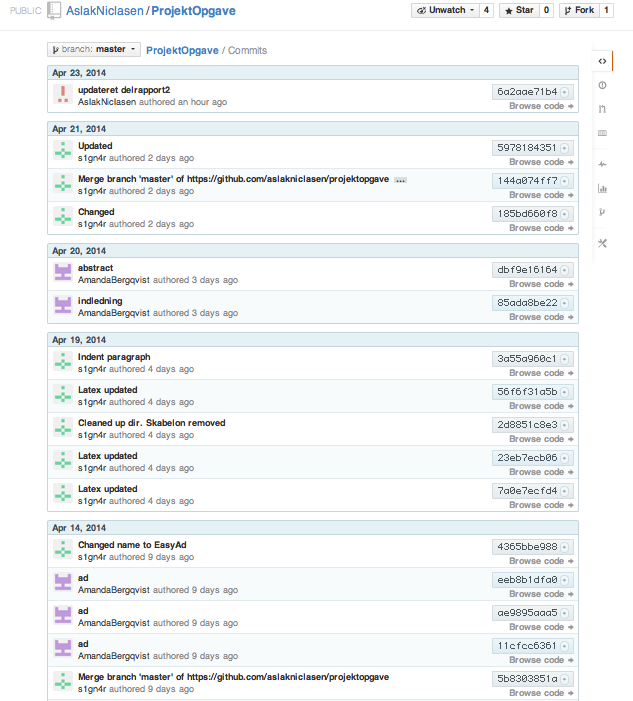
\includegraphics[width=\linewidth]{log1.png}
\newpage
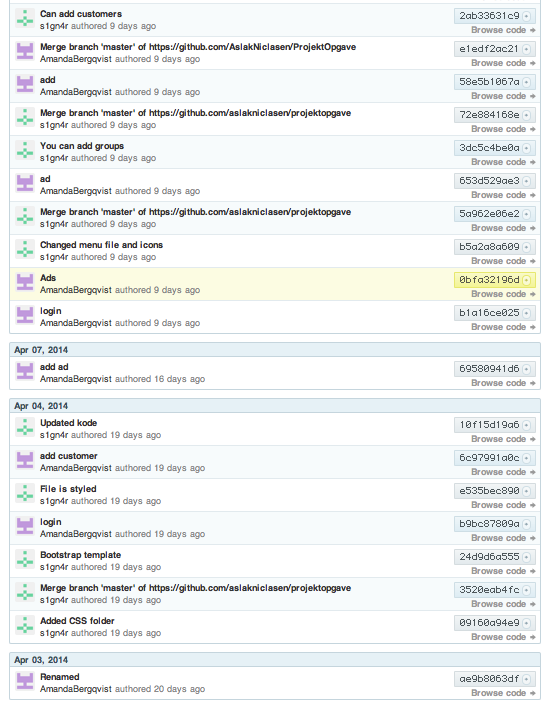
\includegraphics[width=\linewidth]{log2.png}
\newpage
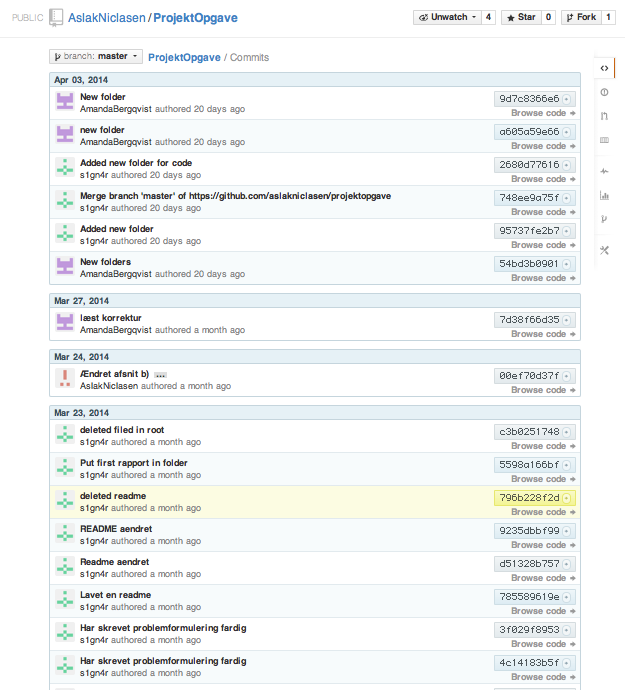
\includegraphics[width=\linewidth]{log3.png}
\newpage
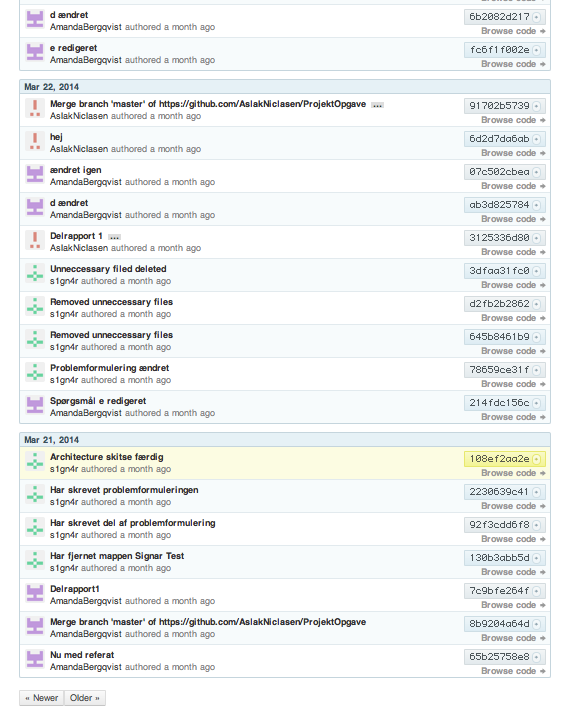
\includegraphics[width=\linewidth]{log4.png}
\newpage
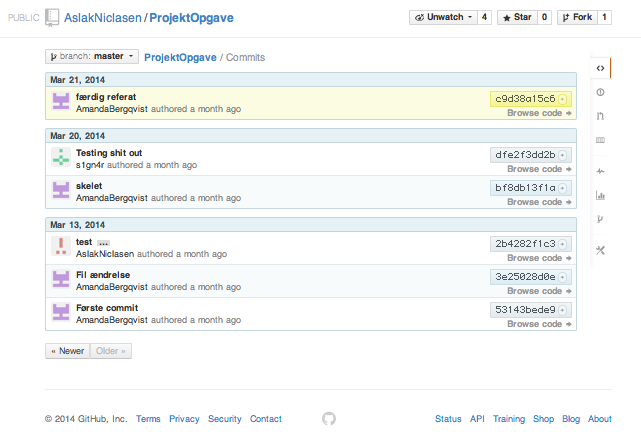
\includegraphics[width=\linewidth]{log5.png}

\end{document}